\documentclass[xcolor={usenames,svgnames,x11names,dvipsnames,table}]{beamer}

\usetheme{SBUclass}
\usepackage{mypackages}
\usepackage{mycommands}

\title{\texorpdfstring{Language \& Technology}{Language and Technology}}
\subtitle{Lecture 2: Dialogue Systems and the Turing Test}
\author{Al{\"e}na Aks{\"e}nova \& Aniello De Santo}
\institute{Stony Brook University\\\texttt{alena.aksenova@stonybrook.edu}\\\texttt{aniello.desanto@stonybrook.edu}}
\date{}


\begin{document}
\unnumbered{
\begin{frame}
	\titlepage
\end{frame}
}

\begin{frame}{Dialogue Systems}
    \begin{columns}
        \column{.6\linewidth}
        \begin{itemize}
            \item system for talking with user
            \item colloquial term: \textbf{chatbot}
        \end{itemize}

        \begin{block}{Possible Uses}
            \begin{itemize}
                \item 24h phone and online support\\
                    \subpoint{Optimum help chat?}
                \item telemarketing\\
                    \subpoint{Samantha West for health insurance}
                \item video games\\
                    \subpoint{Façade, event[0]}
            \end{itemize}
        \end{block}

        \column{.4\linewidth}
        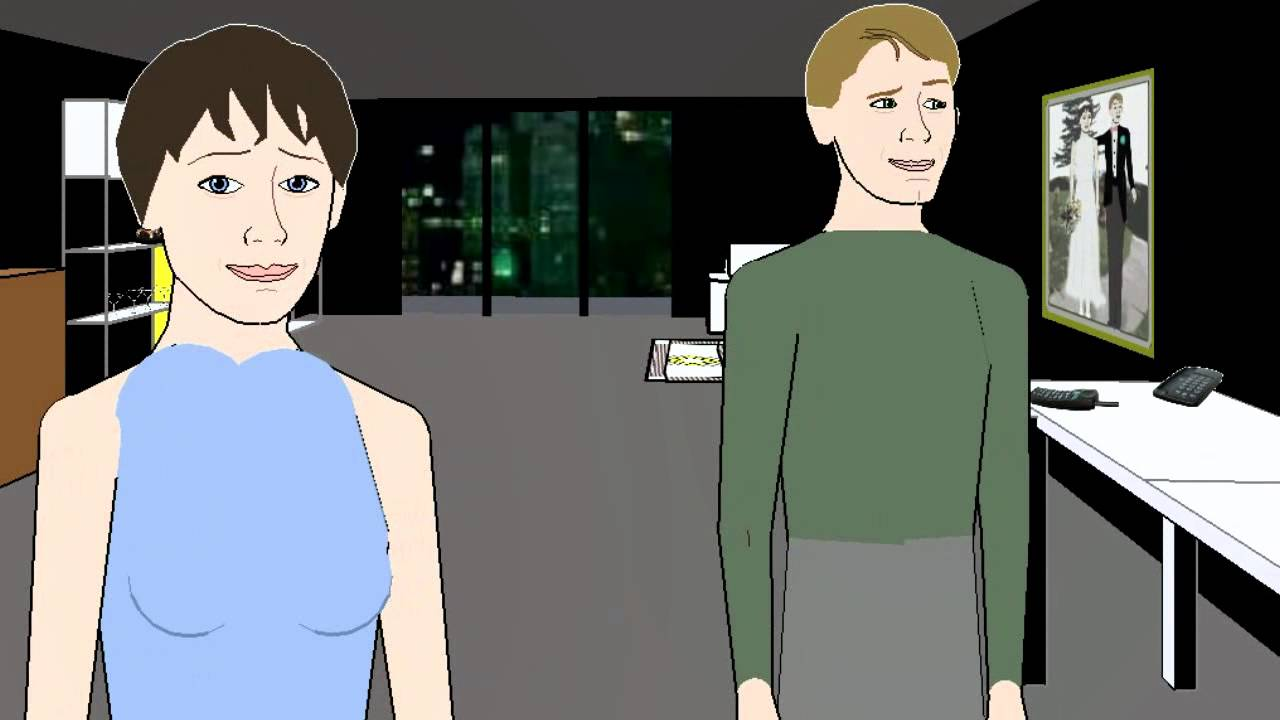
\includegraphics[width=1\linewidth]{./img/facade}\\
        
\includegraphics[width=1\linewidth]{./img/facade2}
    \end{columns}
\end{frame}

\begin{frame}{The First and Most Famous Chatbot: ELIZA}
    \begin{itemize}
        \item developed by Joseph Weizenbaum (MIT) 1964--1966
        \item pretends to be psychotherapist
        \item fooled a surprising number of test subjects
    \end{itemize}

    \begin{block}{ELIZA Effect}
        \begin{itemize}
            \item The tendency of humans to assume computer behavior is\\ analogous to human behavior.
            \item Reading human intentionality into mechanistic symbol manipulations.
        \end{itemize}
    \end{block}

    \pause
    \begin{center}
        Try it yourself: \url{http://www.manifestation.com/neurotoys/eliza.php3}
    \end{center}
\end{frame}


\begin{frame}{How Chatbots ``Cheat''}
    \begin{itemize}
        \item text only, no speech
        \item restricted topic of conversation\\
            \subpoint{medical advise, weather forecast, \ldots}
        \item formulaic or specialized discourse\\
            \subpoint{ordering train tickets, room reservation, \ldots}
        \item grammar with few distinct word forms, restricted word order\\
            \subpoint{English VS German VS Hungarian}
    \end{itemize}
\end{frame}

\begin{frame}{Why Chatbots Need to Cheat}
    \begin{itemize}
        \item Dialog is arguably the \highlight{hardest problem in NLP}.
        \item \textbf{Requires:}
            \begin{itemize}
                \item perfect command of English grammar
                \item analysis of meaning
                \item rich world knowledge
                \item ability to keep track of discourse\\
                    \subpoint{save new information, recall established facts}
                \item correct turn taking
                \item understanding non-literal speech\\
                    \subpoint{indirect speech acts, humor, \ldots}
                \item sophisticated reasoning\\
                    \subpoint{developing and following arguments}
            \end{itemize}
    \end{itemize}
\end{frame}

\begin{frame}{Strategies for Detecting Chatbots}
    \begin{enumerate}[<+->]
        \item \textbf{Be annoying}\\
              Ask the same thing over and over again.\\
              Do you get contradicting replies?
        \item \textbf{Be a giant douche}\\
              Say something that is completely beyond the pale.\\
              Do you get a scolding or shocked reply?
        \item \textbf{Be a polyglot}\\
              Randomly switch languages.\\
              Do you get replies in a matching language,\\
              without any mention of the language change?
        \item \textbf{Be recent}\\
              Incorporate recent events that a human would be aware of.\\
              Do you get a meaningful reply?
        \item \textbf{Be insane}\\
              Ignore all rules of language (word order, grammar, etc.).\\
              Do you get a surprisingly normal reply?
    \end{enumerate}
\end{frame}

\begin{frame}{Let's Try Some of This\ldots}
    Cleverbot: \href{http://www.cleverbot.com/}{http://www.cleverbot.com/}

    \begin{center}
        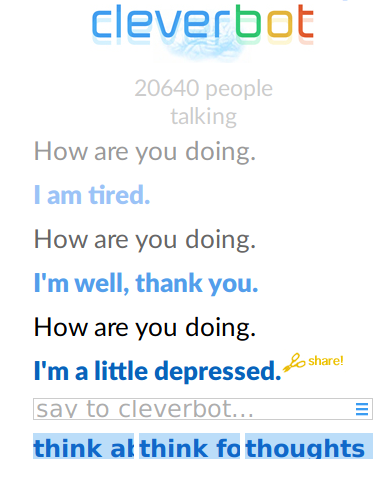
\includegraphics[width=.5\linewidth]{./img/cleverbot.png}
    \end{center}
\end{frame}


\begin{frame}{The Turing Test}
    \begin{columns}
        \column{.7\linewidth}
            \textbf{Alan Turing (1912--1954)}
            \begin{itemize}
                \item British mathematician\slash computer scientist
                \item cracked the \emph{Enigma} in WW2
                \item father of computation (Turing machine)
                \item defined artificial intelligence (Turing test)
                \item extreme long-distance runner (40+ miles)
            \end{itemize}
        \column{.35\linewidth}
        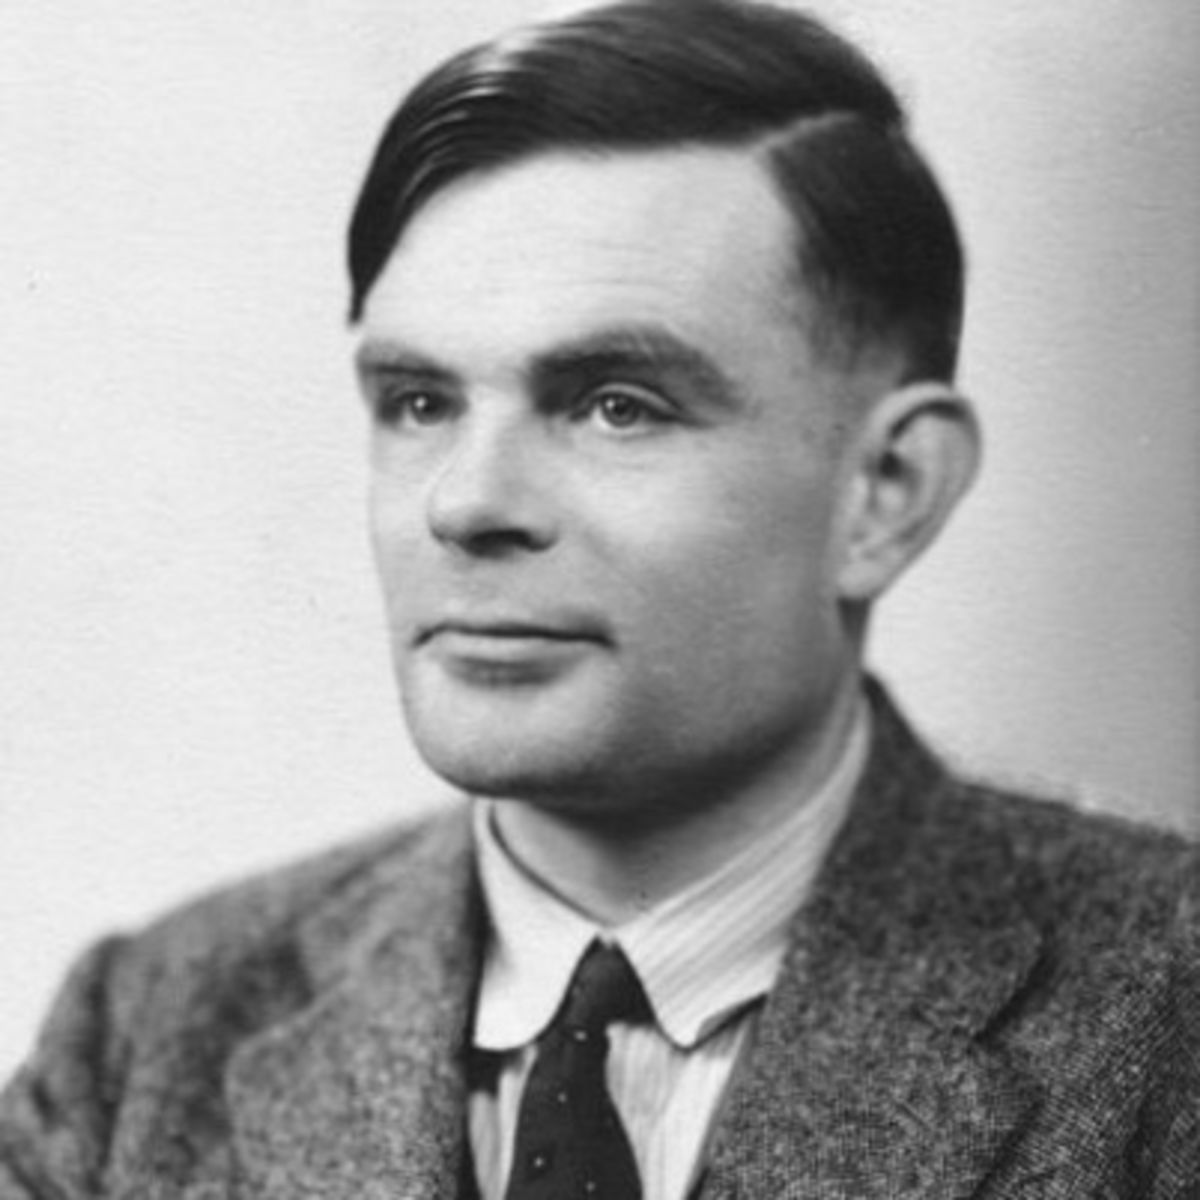
\includegraphics[width=1\linewidth]{./img/turing}
    \end{columns}

    \pause
    \medskip
    \begin{itemize}
        \item Turing was interested in the possibility of artificial intelligence.
        \item What does it mean for a machine to be \highlight{intelligent}?
        \item \textbf{Turing's proposal}\\
            A machine is intelligent if humans \highlight{cannot distinguish it from a human}.
    \end{itemize}
\end{frame}


\begin{frame}{Artificial Intelligence and the Turing Test}
    \begin{block}{Turing Test}
        \begin{itemize}
            \item human C joins remote\slash online chat
            \item must decide whether they are talking to\\
                  human B or machine A
            \item machine A passes test if human C believes it is human
        \end{itemize}
    \end{block}

    \begin{center}
        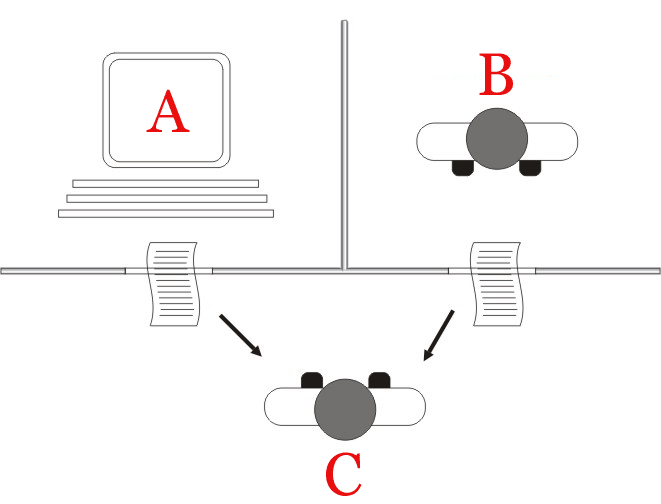
\includegraphics[width=.55\linewidth]{./img/Turing_test_diagram.png}
    \end{center}
\end{frame}

\begin{frame}{Criticism of the Turing Test}
    Some believe the Turing test is \highlight{too weak}.
    
        \begin{block}{Searle's Chinese Room}
            \begin{itemize}
                \item Suppose a person who doesn't speak Chinese is locked into\\ a room full of Chinese phrase books.
                \item To the outsider, the person seems proficient in Chinese. 
                \item appearing intelligent $\neq$ being intelligent
            \end{itemize}
        \end{block}

        \centering
        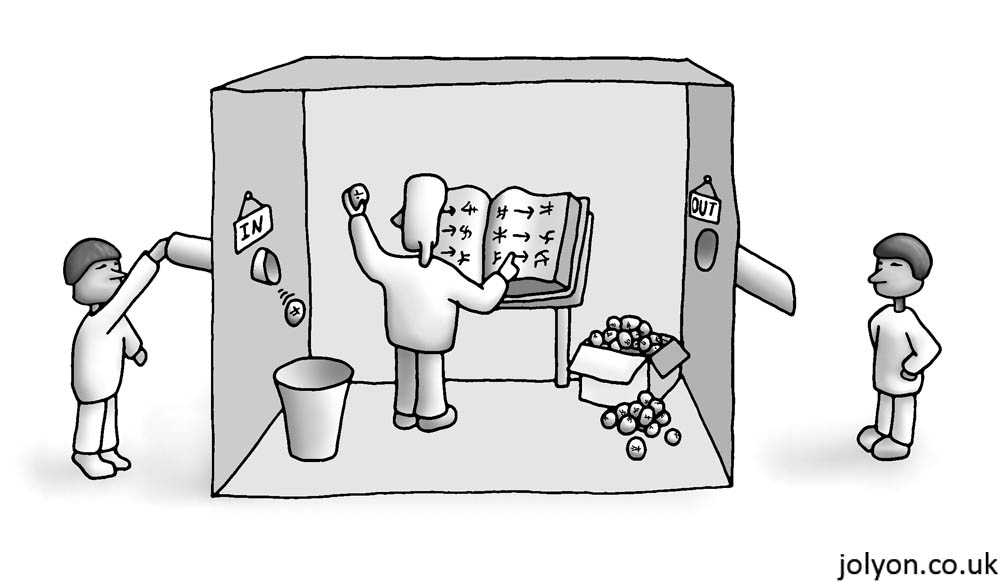
\includegraphics[width=.7\linewidth]{./img/chineseroom}
\end{frame}

\begin{frame}{A Different View}
    I believe the Turing test is \highlight{too strong}.
    %
    \begin{itemize}
        \item intelligence $\neq$ human intelligence
        \item AIs have very different memory and computation abilities.
        \item We should not expect them to think like humans.
        \item Also, humans can fail\slash differ in various aspects of intelligence.\\
            \subpoint{Autism, Williams syndrome, \ldots}
    \end{itemize}

    \pause
    \begin{block}{The Pragmatic Viewpoint}
        \begin{itemize}
            \item In the end, all of this only matters for establishing AI rights.
            \item An AI that is autonomous enough to demand rights is sufficiently intelligent to deserve them.
        \end{itemize}
    \end{block}
\end{frame}

\begin{frame}{(Artificial) Intelligence in the Media}
    \begin{center}
        \begin{tabular}{cccc}
            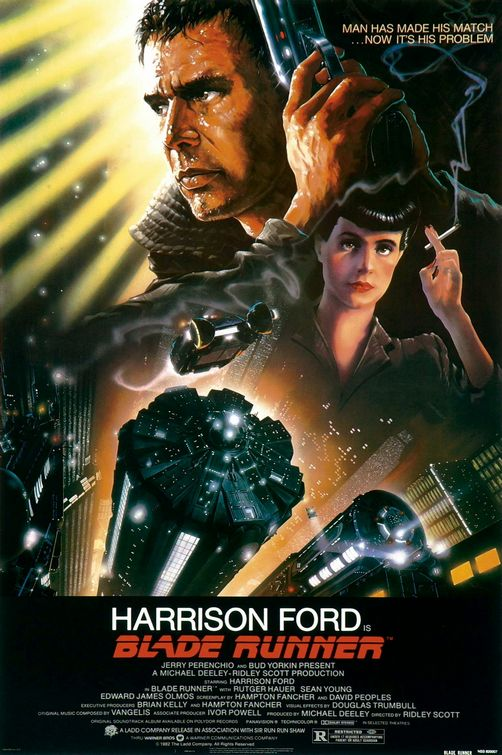
\includegraphics[width=.2\linewidth]{./img/bladerunner}
            &
            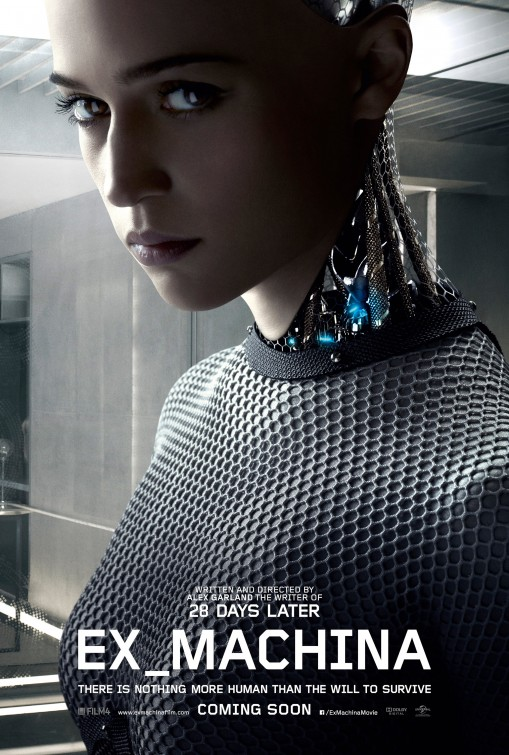
\includegraphics[width=.2\linewidth]{./img/exmachina}
            &
            
\includegraphics[width=.2\linewidth]{./img/ghostintheshell}
            &
            
\includegraphics[width=.2\linewidth]{./img/serialexperimentslain}
            \\
            
\includegraphics[width=.2\linewidth]{./img/startrek1}
            &
            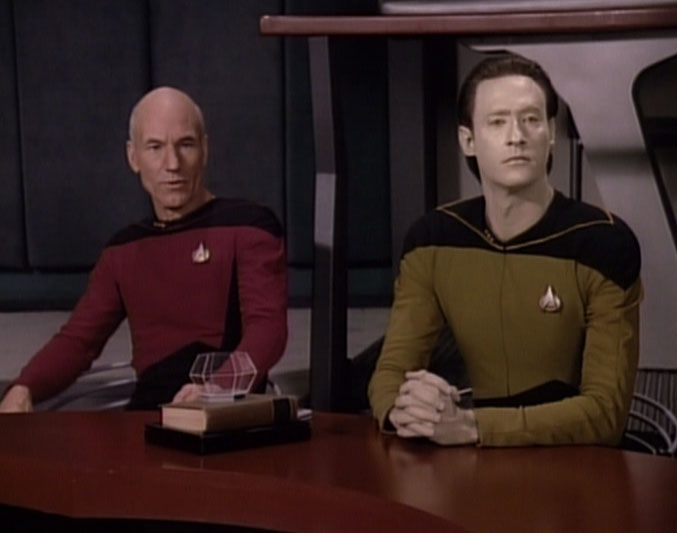
\includegraphics[width=.2\linewidth]{./img/measureofaman}
            &
            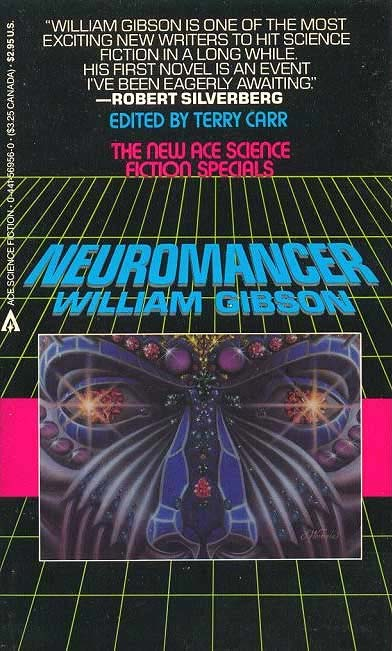
\includegraphics[width=.2\linewidth]{./img/neuromancer}
            &
            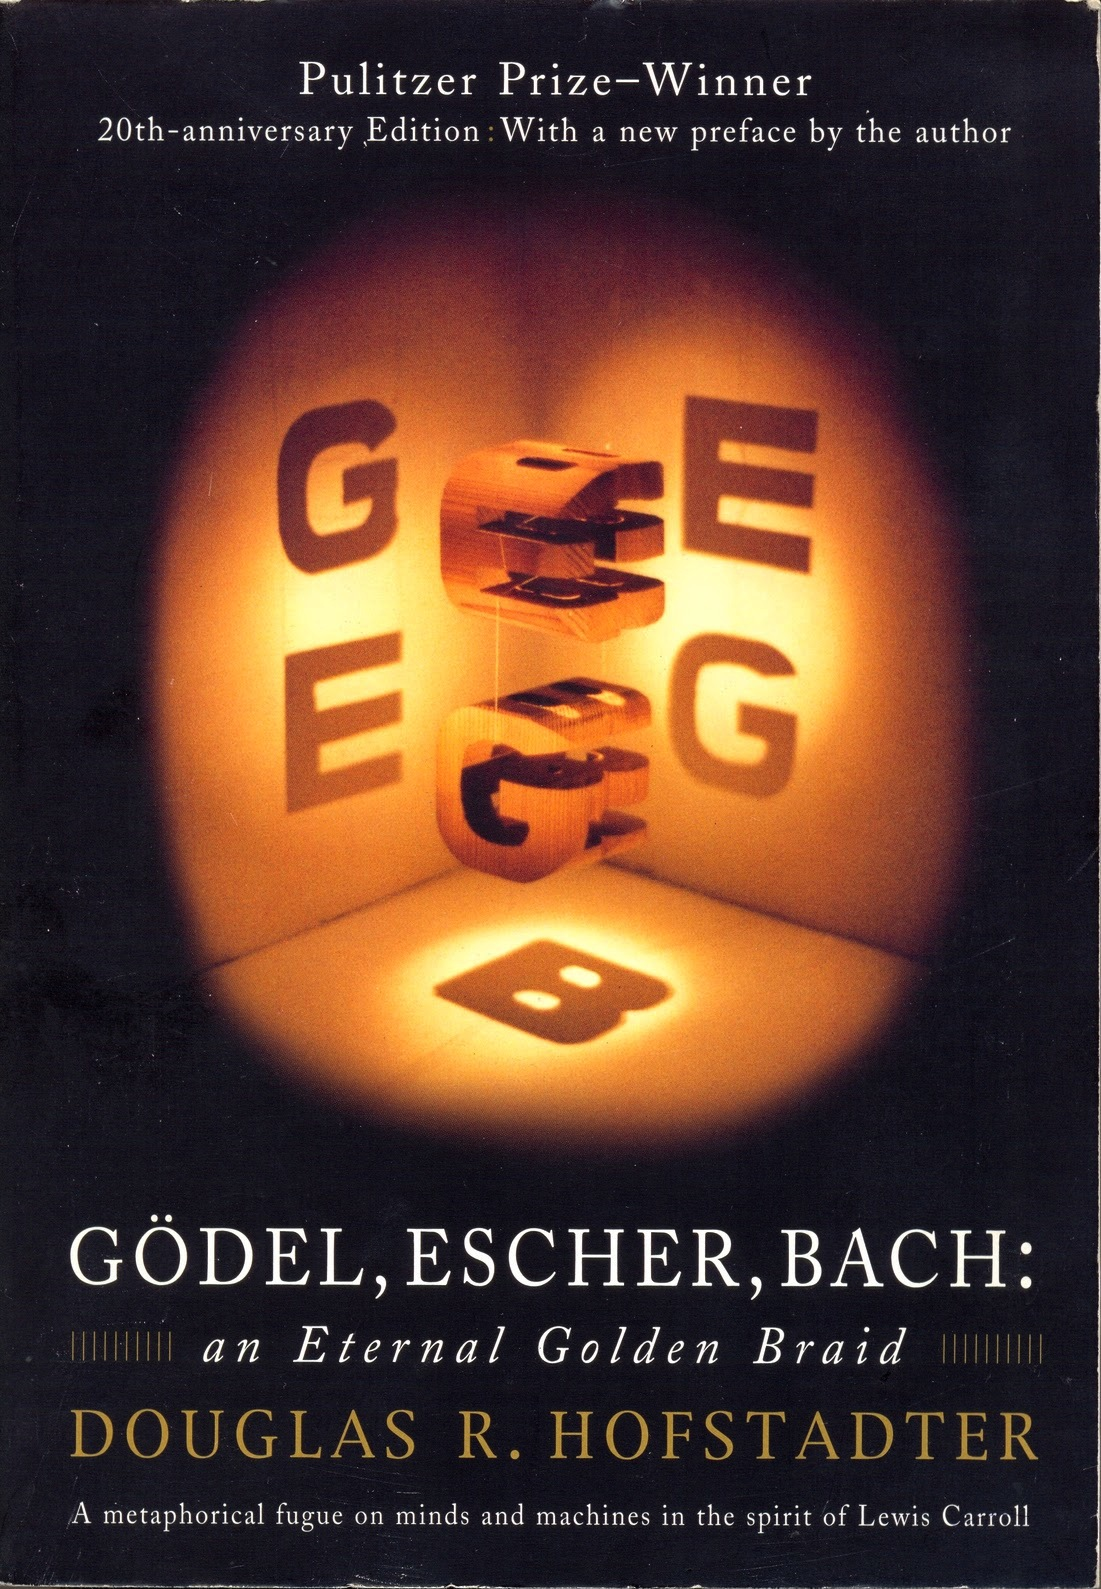
\includegraphics[width=.2\linewidth]{./img/godelescherbach}
        \end{tabular}
    \end{center}
\end{frame}

\begin{frame}{Back to Cleverbot: AI?}
    \begin{center}
     \href{https://www.reddit.com/r/funny/comments/asga0m/two_ai_chatbots_talking_to_each_other_like_old/} {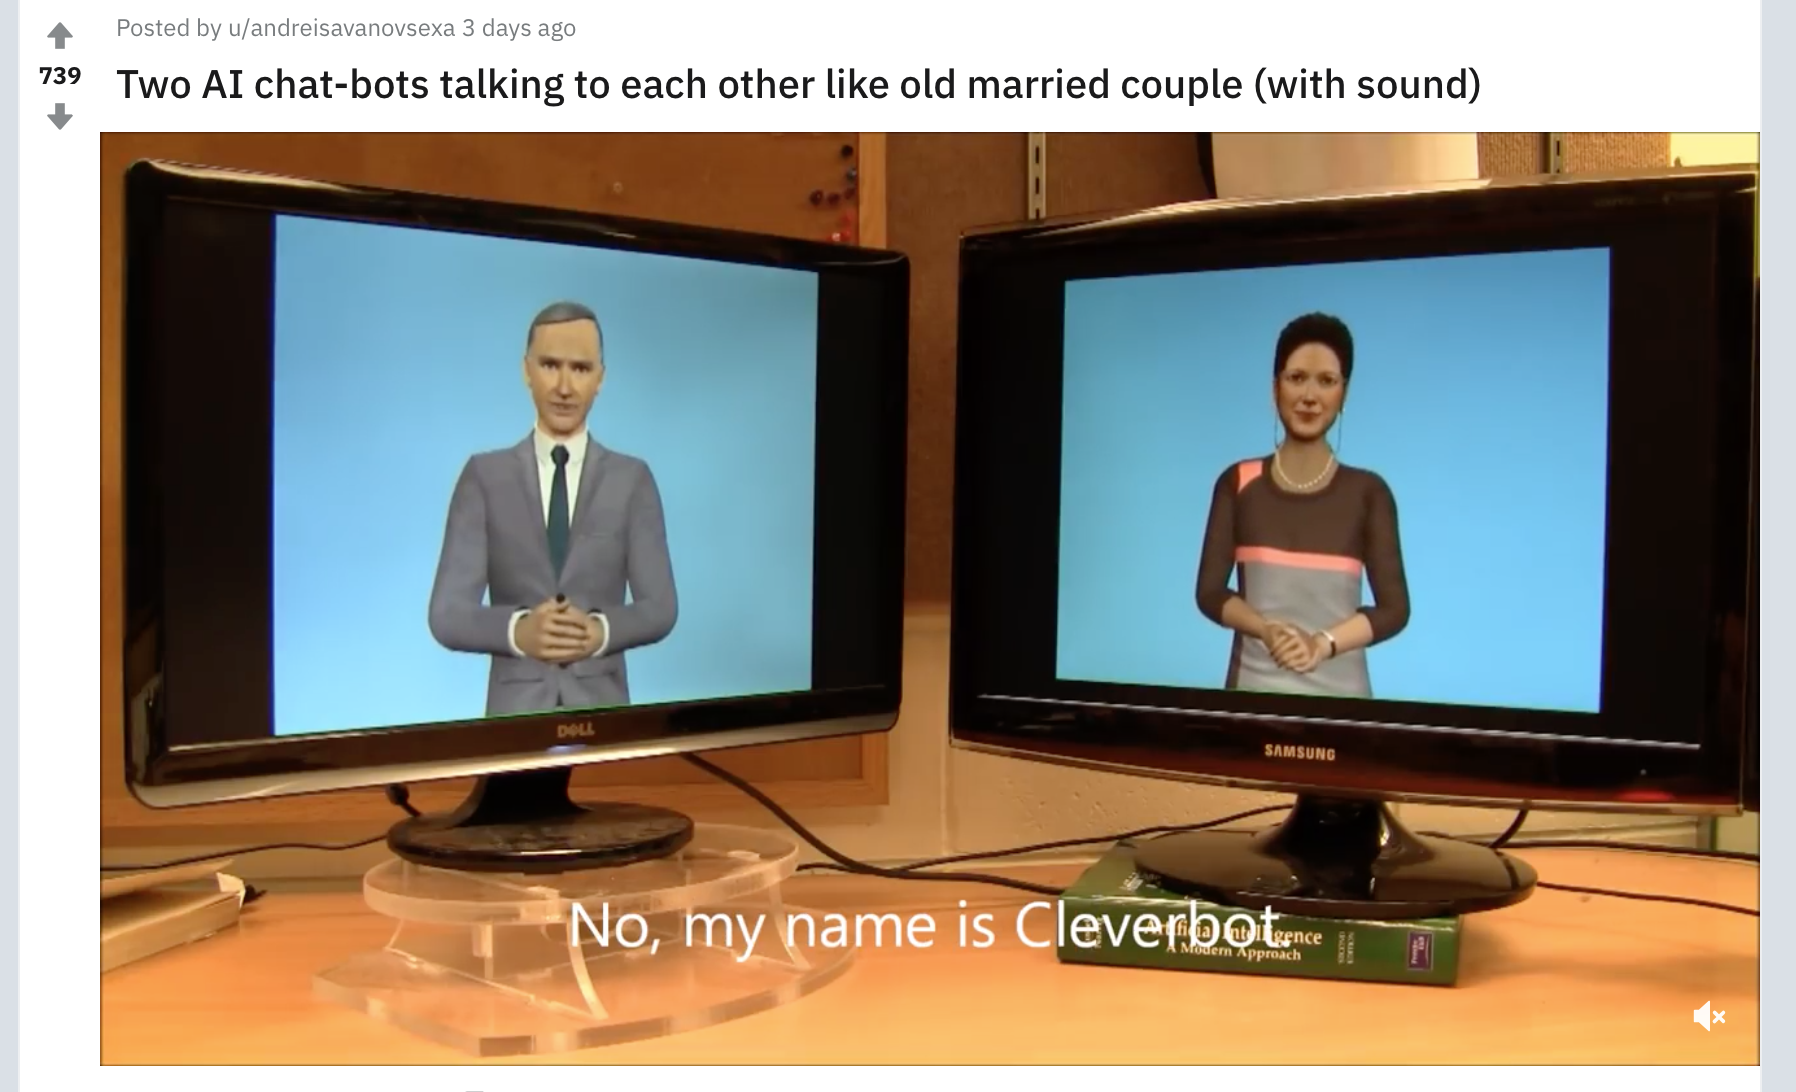
\includegraphics[width=\linewidth]{./img/cleverbotAI}}
     \end{center}
   \end{frame}

\begin{frame}{A Real-World Turing Test: Loebner Prize}
    \begin{itemize}
        \item Loebner Prize: \$3,000 for chatbot that fools human judges
        \item meant as a real-world Turing test
        \item Loebner Prize has been won several times
        \item \textbf{But:} all of the chatbots are just \highlight{tweaked versions of Eliza}
        \item How is this possible?
    \end{itemize}
\end{frame}

\begin{frame}[fragile]{Analyzing ELIZA}
    \begin{itemize}
        \item ELIZA uses pattern matching.
        \item Specific constructions provide specific responses.
    \end{itemize}
    %
    \begin{example}
\begin{pythoncode}
    if 'you' in user_input:
        print('We were discussing you, not me.')
    if 'feel' in user_input:
        print('Tell me more about such feelings.')
\end{pythoncode}
    \end{example}
    %
    \begin{itemize}
        \item Responses can reuse user input with \textbf{regular expressions}\\
              (more on that in a later lecture)
    \end{itemize}
\end{frame}

\begin{frame}{ELIZA's Legacy}
    \begin{itemize}
        \item ELIZA is a simplistic solution for a very complex problem.
        \item With enough tweaking, chatbots work incredibly well\\
            for restricted domains.
        \item Almost all chatbots nowadays thus follow the ELIZA model.
        \item This is a shame, as dialogue systems were meant to be\\
            the vanguard of artificial intelligence.
    \end{itemize}
\end{frame}

\begin{frame}{Experiment: A Mini Turing Test}
    \begin{itemize}
        \item We can't play with Loebner Prize chatbots.\\
              Most of them are not available online.
        \item But we can do a mini-experiment with similar technology:\\
              \highlight{poetry generators}
              \end{itemize}
\pause      
\begin{columns}[T]
    \begin{column}{.4\textwidth}

\begin{block}{Haiku}
\begin{itemize}
\item A very short form of Japanese poetry;
\item three phrases of 5, 7, and 5 syllables;
\item an example by Basho.
\end{itemize}
\end{block}

    \end{column}
    \begin{column}{0.6\textwidth}
   
     \only<3->{
     
\includegraphics[width=0.7\textwidth]{img/haiku}}
      
    \begin{quote}
      \only<3->{
    \small
    	the first cold shower\\
	even the monkey seems to want\\
	a little coat of straw
	}
    \end{quote}

    \end{column}
  \end{columns}
\end{frame}

%              
      \begin{frame}{Let's do it!}
                 \begin{itemize}
        \item The next slides include some Haiku
        \item Some of them were generated by a Python script Al{\"e}na and I wrote.
         \begin{itemize}
        \item note great code, but it does it's job :P
        \end{itemize}
        \item Some are by the famous Japanese poet Basho.
        \item For each one, guess whether it was written by Basho, or Python.
    \end{itemize}
\end{frame}


\begin{frame}{Haiku 1}
    \begin{quote}
\centering
Tomb wherein we tore\\
stem which never knew my life\\
lance of eternal...\\
\end{quote}
    \only<2->{\flushright{[us!]}}
\end{frame}



\begin{frame}{Haiku (2 and 3)}

\begin{columns}[T]
    \begin{column}{.6\textwidth}
   
    \begin{quote}
Lightning flash\\
what I thought were faces\\
are plumes of pampas grass...\\
\only<2->{\flushright{[Basho]}}
    \end{quote}
    \end{column}
        \begin{column}{.6\textwidth}
         \begin{quote}   
            Other thing unknown\\
burnt out the night of yellow\\
hyacinth glory...\\
\only<2->{\flushright{[us!]}}
\end{quote}
        \end{column}
        
        \end{columns}
        \end{frame}
        
        \begin{frame}{Haiku (4 and 5)}
        \begin{columns}[T]
    \begin{column}{.6\textwidth}
   \centering
    \begin{quote}
        Spite of ocean bed\\
sang to the morning bee she\\
sail against the black...\\
\only<2->{\flushright{[us!]}}
\end{quote}
 \end{column}
        \begin{column}{.6\textwidth}
         \begin{quote}

Haste precipitate\\
symmetry of all right in\\
incestuous gloom...\\
\only<2->{\flushright{[us!]}}
\end{quote}
                \end{column}
        
        \end{columns}
\end{frame}

\begin{frame}{Last one!}
\vspace{1cm}
\begin{quote}
\centering
Do not imitate me, \\
Never be like a mush melon \\
Cut in two identical halves. \\
\only<2->{\flushright{\small
[Matsuo Basho]}}
\end{quote}

\end{frame}


%%%%END HAIKU

%\begin{frame}{Poem 1}
%    \small
%    \begin{quote}
%        Try to hold on\\
%        And we have survived\\
%        Try to hold on\\
%        And no one should deny\\
%        We tried to hold on to the pulse of the feedback current\\
%        Into the flow of encrypted movement\\
%        Slapback kills the ancient remnants\\
%        That try to hold on \\
%        Pop tart\\
%        You never listen\\
%        Skinned knees\\
%        Try to hold on\\
%        Stop start\\
%        What's our mission\\
%        Skinned knees\\
%        Try to hold on\\
%    \end{quote}
%\end{frame}
%
%\begin{frame}{Poem 2}
%    \small
%    \begin{quote}
%        a phoenix rising \\
%        from an extremely incriminating photo of us \\
%        friendly reminder\\
%        unrelated side note \\
%        i became pregnant with me\\
%        actually my giant face is nearly sold out of\\
%        irony, sincerity, vagueness, kafka, racism, feminism, kant, buddhism, internet\\
%        names of mind leaping over obstacles set by adults\\
%        reality in my internal universe in transit\\
%        an exhausted observing male teenaged individual \\
%        is the intrepid orange cat\\
%    \end{quote}
%\end{frame}
%
%\begin{frame}{Poem 3}
%    \small
%    \begin{quote}
%        A wounded deer leaps highest,\\
%        I've heard the daffodil\\
%        I've heard the flag to-day\\
%        I've heard the hunter tell;\\
%        'Tis but the ecstasy of death,\\
%        And then the brake is almost done,\\
%        And sunrise grows so near\\
%        sunrise grows so near\\
%        That we can touch the despair and\\
%        frenzied hope of all the ages.\\
%    \end{quote}
%\end{frame}
%
%\begin{frame}{Poem 4}
%    \small
%    \begin{quote}
%        \visible<1->{some men just want to watch the world burn}\\
%        \visible<2->{some men just want to watch the world learn}\\
%        \visible<3->{some men just want breakfast}
%    \end{quote}
%\end{frame}

\begin{frame}{Evaluation}
    \begin{block}{Liked This?}
        For more of this, go to \href{botpoem.com}{\emph{bot or not}} at \url{botpoet.com}
    \end{block}

    \pause
    \begin{itemize}
        \item Writing convincing poems is \textbf{easier} because
            \begin{itemize}
                \item there is no interactivity
                \item poems can be gibberish
            \end{itemize}
        \item But it is also \textbf{harder} because
            \begin{itemize}
                \item there is meter and rhyme,
                \item you need greater stylistic diversity,
                \item you cannot reuse user input.
            \end{itemize}
        \item Given these results, how do you think anybody won the Loebner prize? 
    \end{itemize}
\end{frame}

\begin{frame}{Recent Loebner Prize Winner: Eugene Goostman}
    \begin{itemize}
        \item pretends to be 13 year old boy from Ukraine
       \only<2->{ \item explains:
            \begin{itemize}
                \item broken English
                \item no knowledge of American culture
                \item uncooperative conversation (stubborn child)
                \item random topic changes
            \end{itemize}}
    \end{itemize}

    \begin{block}{The Trick}
        \begin{itemize}
            \item Loebner prize winners fail standards of human intelligence.
            \item Instead, they use social engineering to lower expectations.
        \end{itemize}
    \end{block}
\end{frame}

\begin{frame}{The Loebner Prize Misses the Point}
    \begin{itemize}
        \item The Turing test is meant as a means for testing whether\\
            a very sophisticated machine is truly intelligent.
        \item The chatbots competing for the Loebner prize are obviously\\
            not intelligent since they are just Eliza on steroids.
        \item Passing the Turing test is pointless if
            \begin{itemize}
                \item we already know that the machines aren't intelligent,
                \item passing depends on lowering the evaluation standards. 
            \end{itemize}
        \item Scientifically, the \highlight{Loebner prize is completely worthless}.
    \end{itemize}
\end{frame}

\begin{frame}{Stuart Shieber's Pogo Stick Analogy}
    \begin{columns}
        \column{.6\linewidth}
            \begin{itemize}
                \item Suppose you have a competition for building the first human-powered\\
                    flying machine.
                \item The ambitious flying machines do not get off the ground, while a pogo stick manages to stay in the air for a few seconds.
                \item So from then on people keep improving pogo sticks.
                \item But obviously even the best pogo stick will never allow you to fly.
            \end{itemize}

        \bigskip
        \footnotesize{\textbf{Reference}\\
            \url{http://www.eecs.harvard.edu/~shieber/Biblio/Papers/loebner-rev-html/loebner-rev-html.html}
        }

        \column{.4\linewidth}
            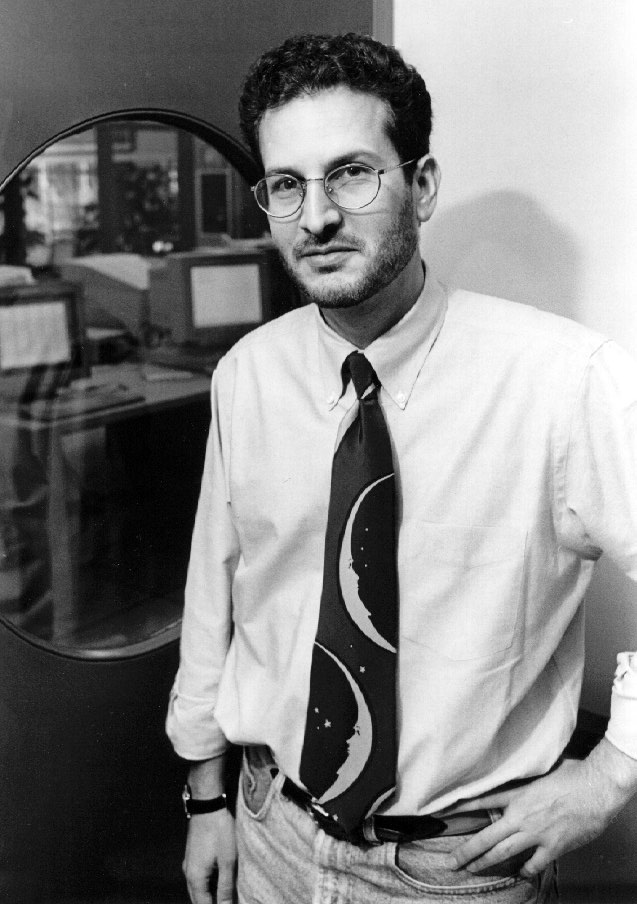
\includegraphics[width=1\linewidth]{./img/shieber}
    \end{columns}
\end{frame}

\begin{frame}{Leaving Pogo Sticks Behind}
    \begin{itemize}
        \item A machine that can pass the Turing test needs\\
            \highlight{genuine understanding of language and the world}.
        \item We are still many years away from that (probably hundreds).
        \item But we can do better than current technology:
            \begin{itemize}
                \item better computational machinery
                \item more linguistic know-how
            \end{itemize}
    \end{itemize}
\end{frame}

\appendix

\unnumbered{
\begin{frame}
    \begin{center}
        \LARGE \bfseries Appendix
    \end{center}
\end{frame}
}

\begin{frame}{More on Alan Turing}
    \begin{columns}
        \column{.7\linewidth}
            \textbf{Alan Turing (1912--1954)}
            \begin{itemize}
                \item British mathematician\slash computer scientist
                \item cracked the \emph{Enigma} in WW2
                \item father of computation (Turing machine)
                \item defined artificial intelligence (Turing test)
                \item extreme long-distance runner (40+ miles)
            \end{itemize}
        \column{.35\linewidth}
        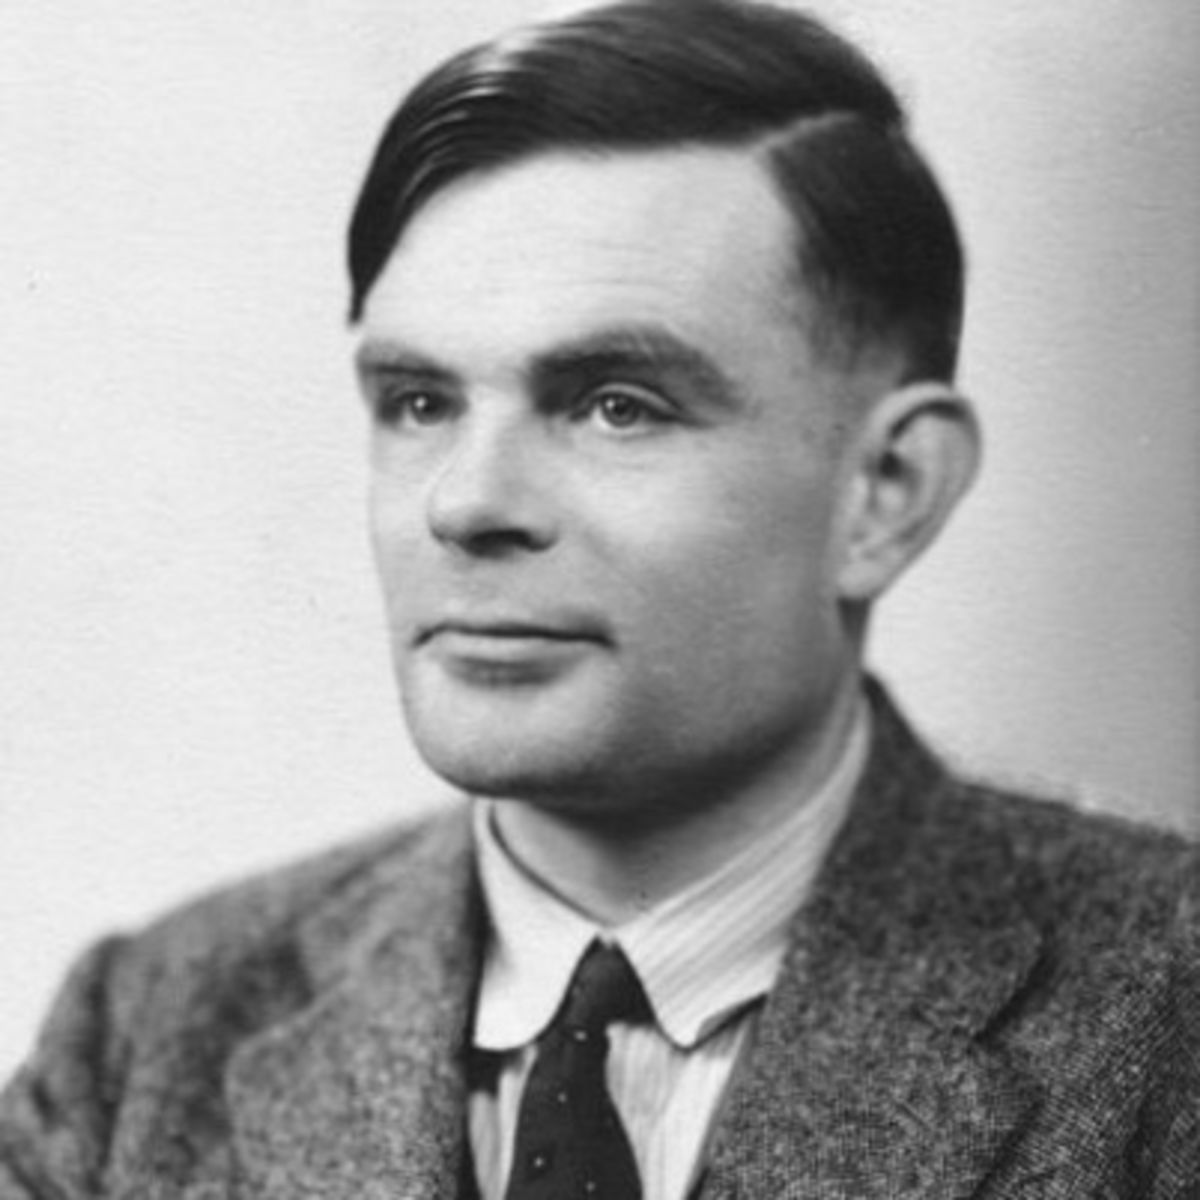
\includegraphics[width=1\linewidth]{./img/turing}
    \end{columns}

    \medskip
    \begin{block}{Tragic Death}
        \begin{itemize}
            \item Turing was gay, a criminal offense in 50s UK.
            \item Turing was sentenced to undergo hormone treatment,\\
                which rendered him impotent and caused severe depression.
            \item Two years later he died of cyanide poisoning\\
                (probably suicide).
        \end{itemize}
    \end{block}
\end{frame}

\begin{frame}{Enigma}
    \begin{columns}
        \column{.5\linewidth}
        \begin{itemize}
            \item Nazi encryption device.
            \item Based on automatic key substitution
            \item Substitution table changed after every key press.
            \item \textbf{Crucial weakness}\\
                Substitutions depend on plugboard configuration\\
                $\Rightarrow$\\
                messages with same configuration use same substitutions
        \end{itemize}

        \column{.5\linewidth}
        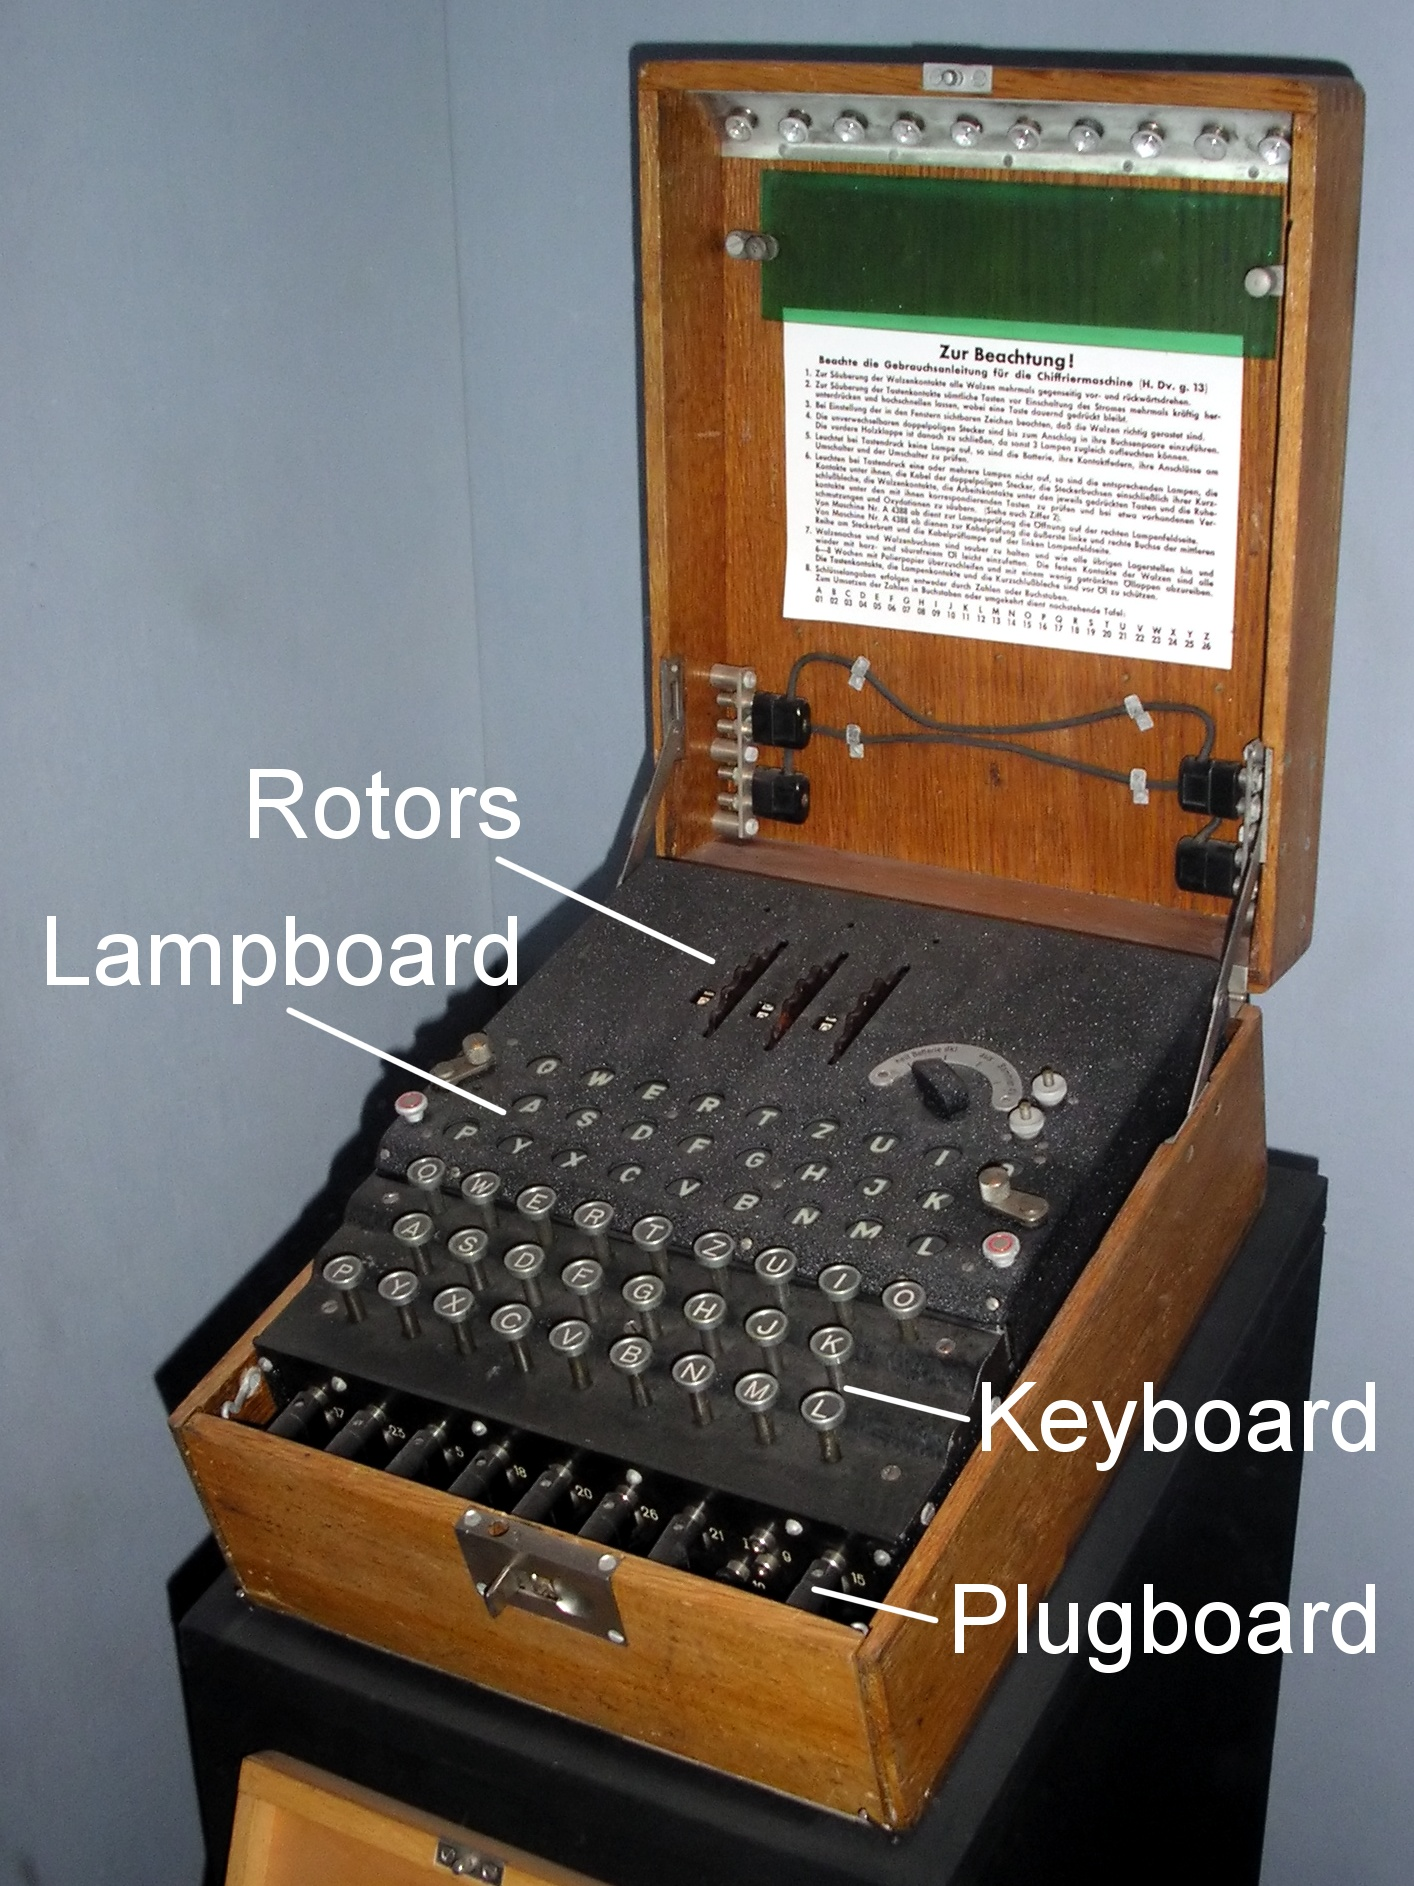
\includegraphics[width=1\linewidth]{./img/enigma}
    \end{columns}
\end{frame}

\begin{frame}{Book\slash Movie Recommendation}
    \begin{columns}
        \column{.6\linewidth}
            \begin{itemize}
                \item long time out of print
                \item recent reprint thanks to movie\\
                    \emph{The Imitation Game}
                \item get it while it lasts
            \end{itemize}
        \column{.4\linewidth}
            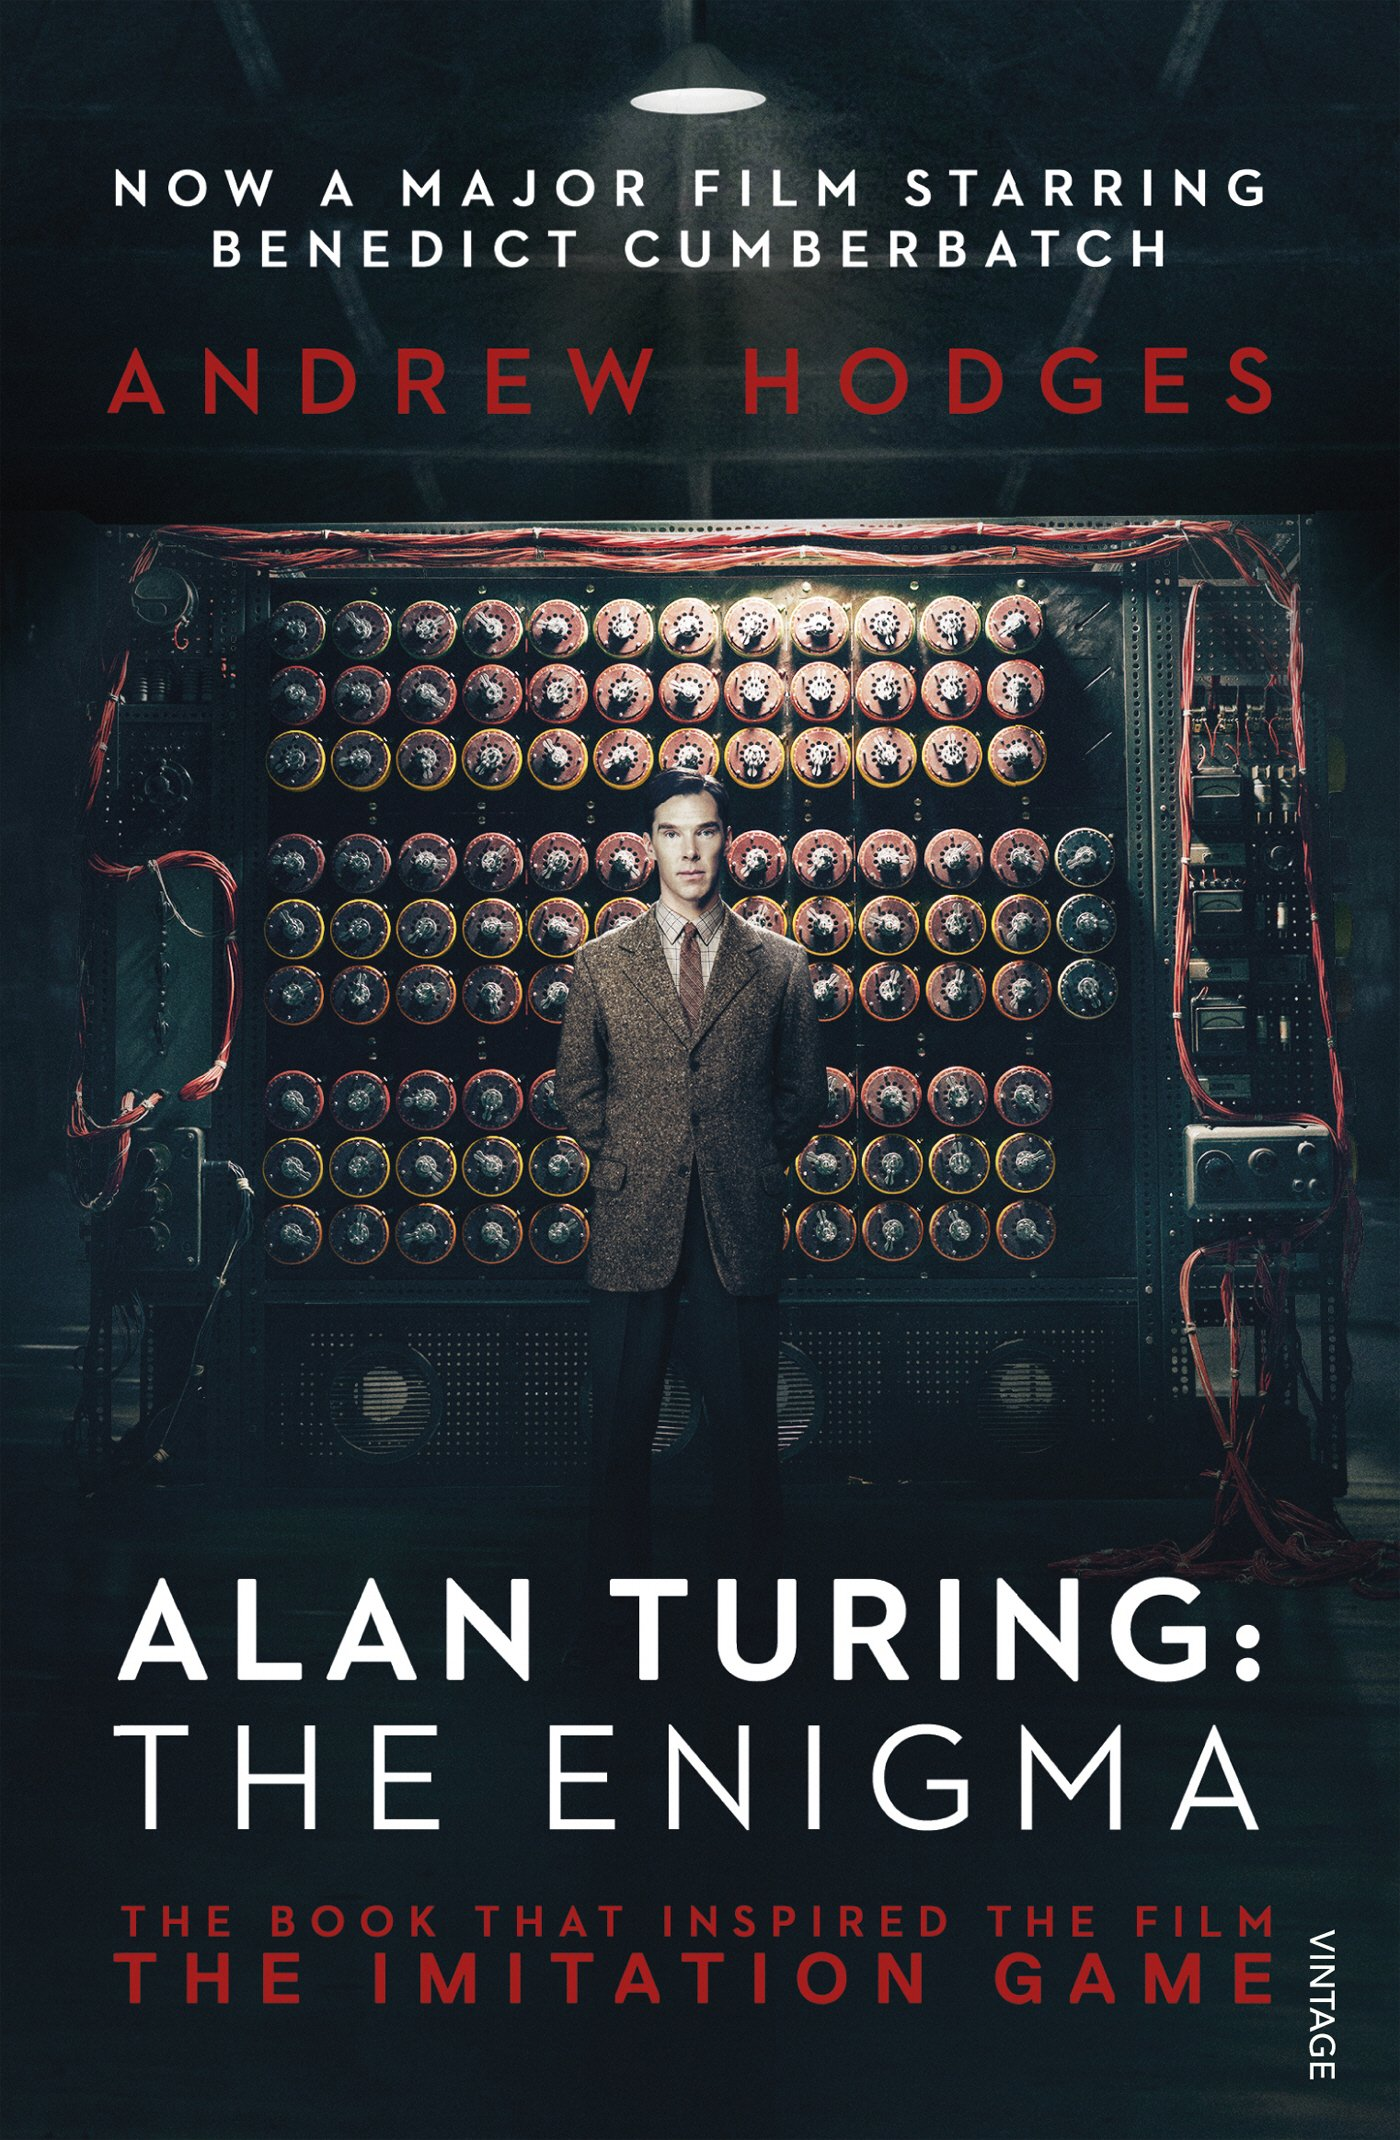
\includegraphics[width=1\linewidth]{./img/enigma_book.jpg}
    \end{columns}
\end{frame}

\begin{frame}{Turing as the Founding Father of Computer Science}
    \emph{On Computable Numbers, with an Application to the Entscheidungs Problem} (1936)

    \begin{block}{What is a Turing Machine?}
        \begin{itemize}
            \item General purpose computing machine
            \item \textbf{Memory:}\\
                    infinite tape that can be filled with symbols
            \item \textbf{Program:}\\
                    finite set of instructions for filling tape with symbols
        \end{itemize}
    \end{block}
\end{frame}

\begin{frame}{Turing Machine}
    \begin{itemize}
        \item Turing machine is abstract, does not specify hardware\\
            \subpoint{tape could be a line of water buckets\ldots}
        \item Function or process is computable if and only if\\ computable by Turing machine
        \item Turing machines are \highlight{universal models of computation}.
        \item Modern-day computers = Turing machines with finite tape
    \end{itemize}
\end{frame}

\begin{frame}{Full Specification of Turing Machine}
    \textbf{Infinite Tape with Read/Write Head and State Register}
    %
    \begin{center}
        \begin{tikzpicture}
            \draw[blue!75,step=2em] (0,0) grid (16em,2em);
            \foreach \y in {0,2}
            {
                \draw[blue!75] (-1em,\y em) to (0em,\y em);
                \draw[blue!75] (16em,\y em) to (17em,\y em);
            }

            \draw[SeaGreen4,fill=SeaGreen4!75,opacity=.5] (9em,.25em) -- (11em,-2em) -- (7em,-2em) -- cycle;
            \node at (9em,-1.25em) {$q$};
        \end{tikzpicture}
    \end{center}

    \bigskip
    \textbf{Instruction Table}
    \begin{center}
        \begin{tabular}{cc|ccc}
            \emph{state} & \emph{tape symbol} & \emph{write action}        & \emph{move action} & \emph{new state}\\
            \hline
                         &                    & delete symbol \emph{or}    & left \emph{or}     & \\
                         &                    & write new symbol \emph{or} & right \emph{or}    & \\
                         &                    & do nothing                 & stay               & 
        \end{tabular}
    \end{center}
\end{frame}

\begin{frame}{Example of Turing Machine}
    \textbf{Instruction Table}
    \begin{center}
        \footnotesize
        \begin{tabular}{cc|ccc}
            \emph{state} & \emph{tape symbol} & \emph{write action} & \emph{move action} & \emph{new state}\\
            \hline
            A            & 0                  & none                & none               & done\\
            A            & 1                  & print(0)            & $\Leftarrow$       & B\\
            B            & 0                  & none                & $\Leftarrow$       & C\\
            B            & 1                  & none                & $\Leftarrow$       & B\\
            C            & 0                  & print(1)            & $\Rightarrow$      & D\\
            C            & 1                  & none                & $\Leftarrow$       & C\\
            D            & 0                  & none                & $\Rightarrow$      & E\\
            D            & 1                  & none                & $\Rightarrow$      & D\\
            E            & 0                  & print(1)            & $\Leftarrow$       & A\\
            E            & 1                  & none                & $\Rightarrow$      & E\\
        \end{tabular}
    \end{center}

    \begin{center}
        \only<2>{
            \begin{tabular}{ccccccccccc}
                0 & 0 & 0 & 0 & 1 & 1 & 0 & 0 & 0 & 0 & 0\\
                  &   &   &   &   & \color{SteelBlue4} A
            \end{tabular}
        }%
        \only<3>{
            \begin{tabular}{ccccccccccc}
                0 & 0 & 0 & 0 & 1 & 0 & 0 & 0 & 0 & 0 & 0\\
                  &   &   &   &   & \color{SteelBlue4} A
            \end{tabular}
        }%
        \only<4>{
            \begin{tabular}{ccccccccccc}
                0 & 0 & 0 & 0 & 1 & 0 & 0 & 0 & 0 & 0 & 0\\
                  &   &   &   & \color{SteelBlue4} B
            \end{tabular}
        }%
        \only<5>{
            \begin{tabular}{ccccccccccc}
                0 & 0 & 0 & 0 & 1 & 0 & 0 & 0 & 0 & 0 & 0\\
                  &   &   & \color{SteelBlue4} B
            \end{tabular}
        }%
        \only<6>{
            \begin{tabular}{ccccccccccc}
                0 & 0 & 0 & 0 & 1 & 0 & 0 & 0 & 0 & 0 & 0\\
                  &   & \color{SteelBlue4} C
            \end{tabular}
        }%
        \only<7>{
            \begin{tabular}{ccccccccccc}
                0 & 0 & 1 & 0 & 1 & 0 & 0 & 0 & 0 & 0 & 0\\
                  &   & \color{SteelBlue4} C
            \end{tabular}
        }%
        \only<8>{
            \begin{tabular}{ccccccccccc}
                0 & 0 & 1 & 0 & 1 & 0 & 0 & 0 & 0 & 0 & 0\\
                  &   &   & \color{SteelBlue4} D
            \end{tabular}
        }%
        \only<9>{
            \begin{tabular}{ccccccccccc}
                0 & 0 & 1 & 0 & 1 & 0 & 0 & 0 & 0 & 0 & 0\\
                  &   &   &   & \color{SteelBlue4} E
            \end{tabular}
        }%
        \only<10>{
            \begin{tabular}{ccccccccccc}
                0 & 0 & 1 & 0 & 1 & 0 & 0 & 0 & 0 & 0 & 0\\
                  &   &   &   &   & \color{SteelBlue4} E
            \end{tabular}
        }%
        \only<11>{
            \begin{tabular}{ccccccccccc}
                0 & 0 & 1 & 0 & 1 & 1 & 0 & 0 & 0 & 0 & 0\\
                  &   &   &   &   & \color{SteelBlue4} E
            \end{tabular}
        }%
        \only<12>{
            \begin{tabular}{ccccccccccc}
                0 & 0 & 1 & 0 & 1 & 1 & 0 & 0 & 0 & 0 & 0\\
                  &   &   &   & \color{SteelBlue4} A
            \end{tabular}
        }%
        \only<13>{
            \begin{tabular}{ccccccccccc}
                0 & 0 & 1 & 0 & 0 & 1 & 0 & 0 & 0 & 0 & 0\\
                  &   &   &   & \color{SteelBlue4} A
            \end{tabular}
        }%
        \only<14>{
            \begin{tabular}{ccccccccccc}
                0 & 0 & 1 & 0 & 0 & 1 & 0 & 0 & 0 & 0 & 0\\
                  &   &   & \color{SteelBlue4} B
            \end{tabular}
        }%
        \only<15>{
            \begin{tabular}{ccccccccccc}
                0 & 0 & 1 & 0 & 0 & 1 & 0 & 0 & 0 & 0 & 0\\
                  &   & \color{SteelBlue4} C
            \end{tabular}
        }%
        \only<16>{
            \begin{tabular}{ccccccccccc}
                0 & 0 & 1 & 0 & 0 & 1 & 0 & 0 & 0 & 0 & 0\\
                  & \color{SteelBlue4} C
            \end{tabular}
        }%
        \only<17>{
            \begin{tabular}{ccccccccccc}
                0 & 1 & 1 & 0 & 0 & 1 & 0 & 0 & 0 & 0 & 0\\
                  & \color{SteelBlue4} C
            \end{tabular}
        }%
        \only<18>{
            \begin{tabular}{ccccccccccc}
                0 & 1 & 1 & 0 & 0 & 1 & 0 & 0 & 0 & 0 & 0\\
                  &   & \color{SteelBlue4} D
            \end{tabular}
        }%
        \only<19>{
            \begin{tabular}{ccccccccccc}
                0 & 1 & 1 & 0 & 0 & 1 & 0 & 0 & 0 & 0 & 0\\
                  &   &   & \color{SteelBlue4} D
            \end{tabular}
        }%
        \only<20>{
            \begin{tabular}{ccccccccccc}
                0 & 1 & 1 & 0 & 0 & 1 & 0 & 0 & 0 & 0 & 0\\
                  &   &   &   & \color{SteelBlue4} E
            \end{tabular}
        }%
        \only<21>{
            \begin{tabular}{ccccccccccc}
                0 & 1 & 1 & 0 & 1 & 1 & 0 & 0 & 0 & 0 & 0\\
                  &   &   &   & \color{SteelBlue4} E
            \end{tabular}
        }%
        \only<22>{
            \begin{tabular}{ccccccccccc}
                0 & 1 & 1 & 0 & 1 & 1 & 0 & 0 & 0 & 0 & 0\\
                  &   &   & \color{SteelBlue4} A
            \end{tabular}
        }
    \end{center}
\end{frame}

\begin{frame}{Another Book Recommendation}
    \begin{columns}
        \column{.6\linewidth}
            \begin{itemize}
                \item friendly intro to Turing machines
                \item development of computers after Turing's initial paper
                \item in particular origins at\\
                    Manhattan project in Los Alamos
            \end{itemize}
        \column{.4\linewidth}
            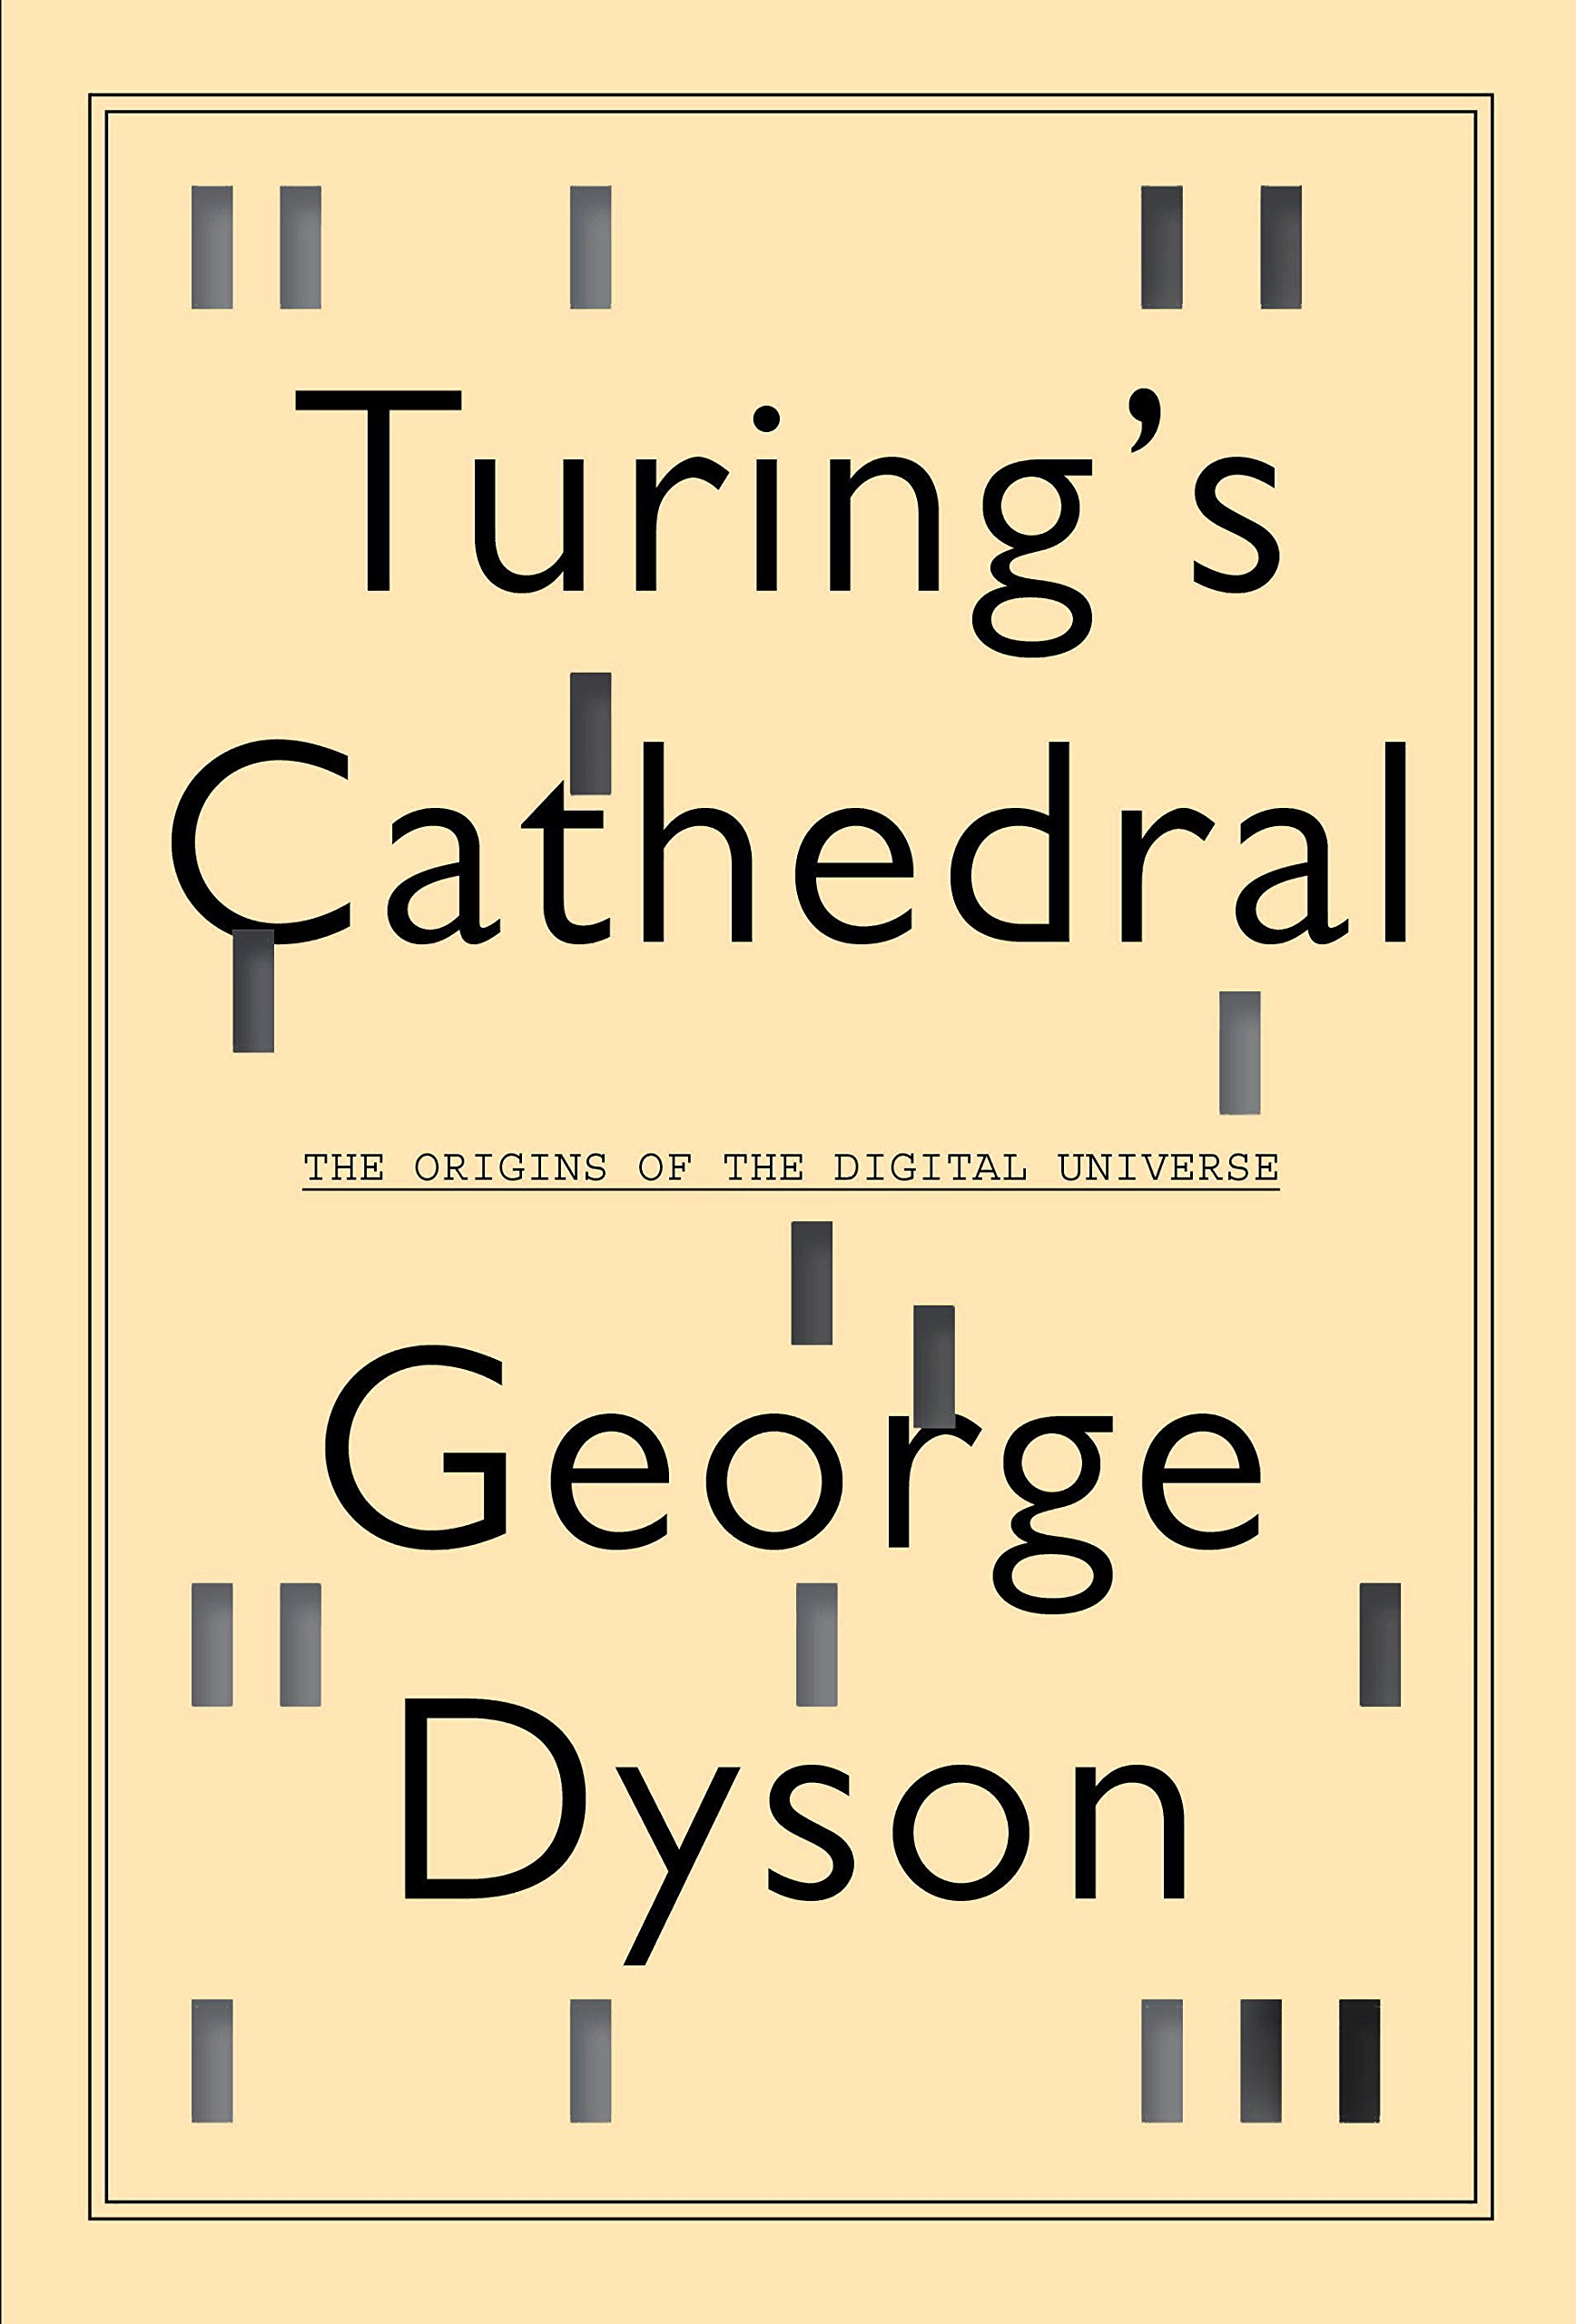
\includegraphics[width=1\linewidth]{./img/turings_cathedral.jpg}
    \end{columns}
\end{frame}

\end{document}
